\documentclass[a4paper, amsfonts, amssymb, amsmath, reprint, showkeys, nofootinbib, twoside]{revtex4-1}

\usepackage[english]{babel}
\usepackage[utf8]{inputenc}
\usepackage[colorinlistoftodos, color=green!40, prependcaption]{todonotes}
\usepackage{graphicx}
\usepackage{subcaption}
\usepackage{float}
\usepackage[bottom]{footmisc}
\usepackage{enumitem}
\usepackage{hyperref}

\bibliographystyle{apsrev4-1}
\setlist{noitemsep}

\begin{document}

\title{%
  \large{Vipassana for Hackers} \\
  \Huge{Paper Three: Why Meditate?} \\
  \large\textit{Version 0.1}
}
\author{Steven Deobald}
\email[Correspondence email address: ]{steven@deobald.ca}
\affiliation{www.vipassana-for-hackers.org}
\date{\today}

\begin{abstract}
 Meditation requires a time commitment. Like other activities we consider
 worthy of our time for their benefits to our health, such as sufficient sleep, exercise, fresh air, and a
 healthy diet, it is often the (rational) first step of individuals considering a
 meditation practice to ask: Why should I bother? What are the outcomes of
 meditation? And do the benefits of those outcomes outweigh the time meditation
 costs the practitioner? This paper answers those questions as they pertain to
 meditation in general, and to Vipassana, specifically.
\end{abstract}

\keywords{neuroplasticity}

\maketitle


\section{Target Audience}

\textit{Vipassana for Hackers, Paper One: Curious Mechanics} was written with the
explicit intention of avoiding a discussion about the specific
outcomes or consequences of meditation in detail. That paper was intentionally,
though artificially, restricted to
the internal mechanics of Vipassana meditation, to pique the interest of potential
meditators who had heard of Vipassana elsewhere. Outcomes are discussed only so far
as they assist the reader in understanding what is written earlier in the paper
regarding human sensory experience. \textit{Paper Two: The Brain} goes further into the internal
mechanics as they pertain to the
hub of the nervous system. In the second paper, outcomes are discussed as they pertain to
neuroplasticity. Neither paper directly discusses why an individual might choose to
try this particular technique of meditation.

As before, the ``Hacker'' of \textit{Vipassana for Hackers} is not meant to identify
computer programmers. Instead, it is meant as a label for a culture of curious and
creative people who enjoy exploring, learning, and creating. Librarians, scientists,
musicians, architects, medical practitioners, carpenters, artists, lovers of books,
mechanics, journalists, academics,
hobbyists of all stripes --- all ``hackers'', of a sort. If you think you belong
here, you do.

\textit{Paper Three: Why Meditate?} is written for anyone who has ever asked
themselves that very question or asked this question of a friend who
meditates. It is for both those who are curious about the practice of Vipassana
specifically and those who are curious about meditation in general. It is for people
who have meditated in other traditions and are curious about the benefits of
Vipassana. It is also for people who have never meditated in their entire lives. It
is intended for anyone who keeps hearing about Vipassana meditation --- in the media,
in books, and from friends --- and wants to learn what all the fuss is about.

The reader need not have read \textit{Paper One} or \textit{Paper Two}. In fact, it
is the intention of this paper to be the most accessible of the series. Readers
with only a faint interest in the topic of meditation should start here.


\section{The Mundane vs. The Supramundane}

There are two fields of human experience and the following analysis of the value
provided by different meditation techniques will break down all points into these two
categories. \textit{The Mundane}
in this context refers not to the tedious but to the earthly, the material. Most people will begin
meditating for reasons in the mundane field simply because most people have never
experienced the supramundane field. \textit{The Supramundane} in this context refers not to
spirituality or religion but experiences which transcend the material, physical
world. Put another way, mundane experiences are those which can be
described. Supramundane experiences, due to their very nature of transcending the
material world, are ineffable. Just because an experience is ineffable, however, does
not mean conversation cannot exist around it. An experience of dimethyltryptamine
(DMT) may be ineffable but it is almost a guarantee that someone using this drug will
talk about it afterward. In this way, we will discuss the consequences of
supramundane experiences (and their value) toward the end of this paper.

Because supramundane experiences tend to occur only in deep meditative states,
the reasons for meditating listed will predominantly fall in the mundane
category. Whether or not the meditator experiences supramundane states in deep
meditation, these altered states of mind are never the goal of meditation. The goal
of meditation is to change the meditator's mental habits. The intention is to move away from unhealthy
mental patterns --- those which cause harmful behaviours --- toward healthy mental patterns which
encourage productive behaviour. Obviously this change is only visible in the mundane
world, outside of meditation.

In \textit{Paper One: Curious Mechanics}, two sample spectrums of meditations were
listed. One included activities which were simply meditative, rather than anything
which could be considered a formal meditation practice. These included sports,
playing a musical instrument, or yogic practices such as asanas and pranayams. We
will ignore such activities here. The following plane attempts to roughly locate
meditation practices between focus and insight on two axes, rather than one.

\begin{figure}[H]
  \centering
  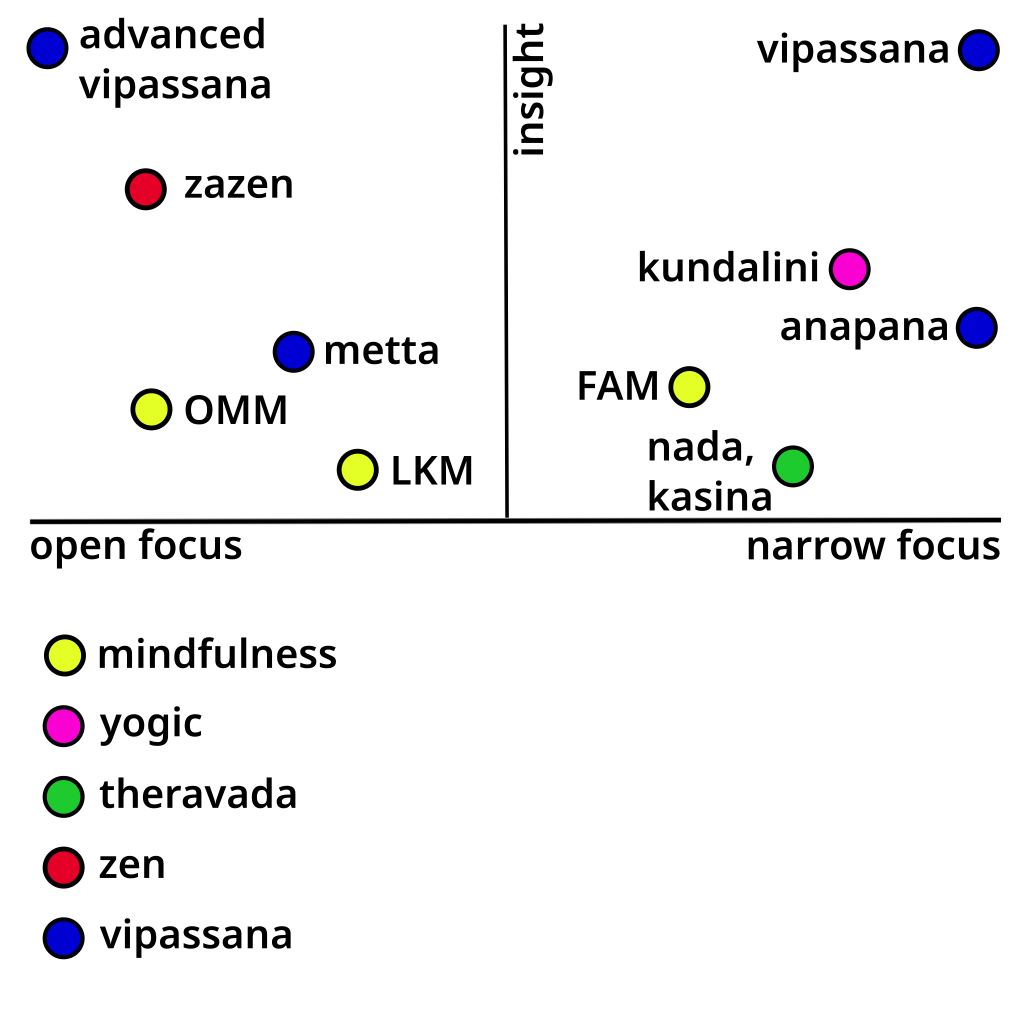
\includegraphics[width=5cm]{images/focus-insight-plane.png}
  \caption{Meditation Quadrants}
  \label{fig:meditation-quadrants}
\end{figure}

The locations of different meditation practices on the graph are only for
illustrative purposes. There are many other axes available such as a practitioner's
experience level, intensity of practice, and an individual's physiology and mental
health. However, this plane helps ground a comparison of different meditation
techniques for the rest of the paper. The three mindfulness meditation categories are
Focused Attention Meditation (FAM), Open Monitoring Meditation (OMM), and
Loving-Kindness Meditation (LKM). These will be explained as mindfulness meditations
come up in discussion later.

Returning to the topic of the supramundane, the following spectrum illustrates where
each of these practices approximately falls, across that dichotomy.

\begin{figure}[H]
  \centering
  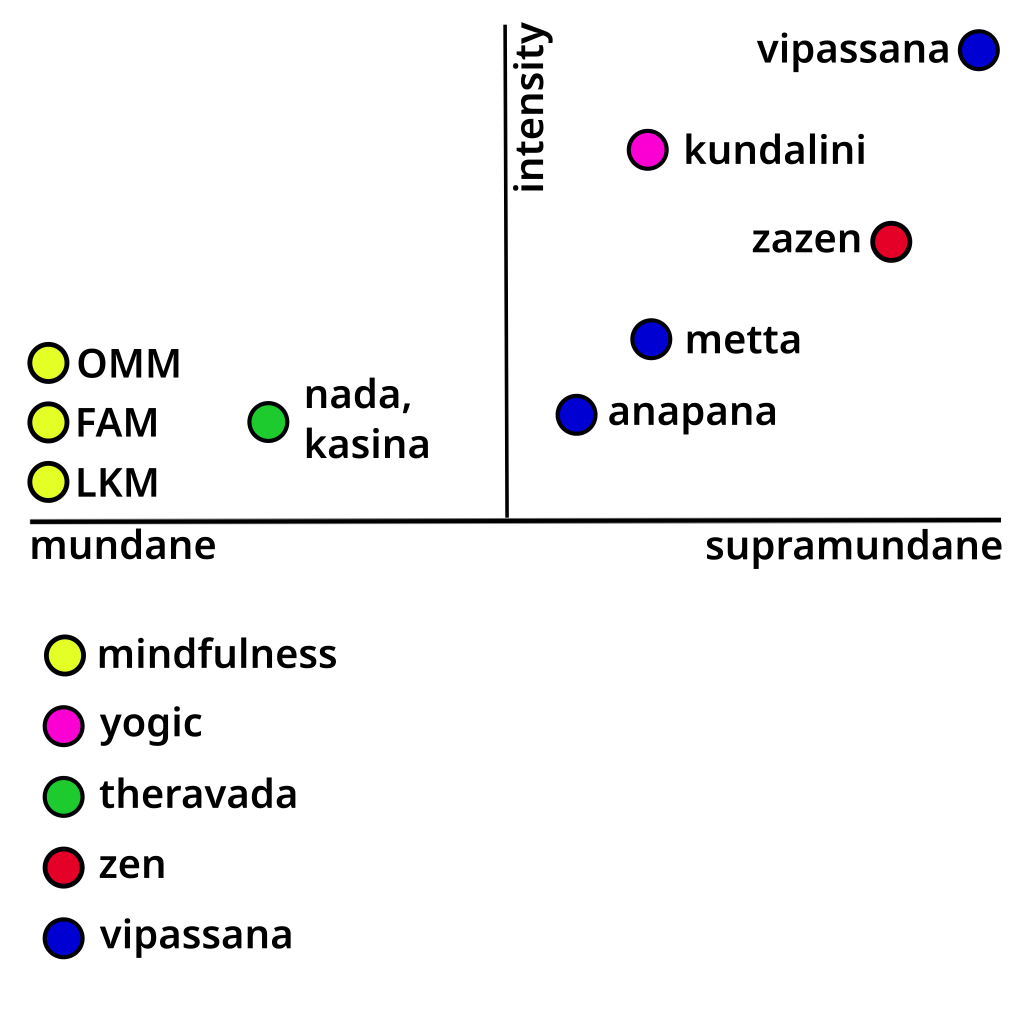
\includegraphics[width=5cm]{images/mundane-supramundane-plane.png}
  \caption{Mundane vs. Supramundane Meditations}
  \label{fig:mundane-vs-supramundane}
\end{figure}

Meditations within the mundane sphere are easier to understand and easier to
teach. As a consequence, they are easier to submit to rigorous scientific
study. Where the broad categories of FAM, OMM, and LKM have been studied
scientifically, we will observer respective parallels in Anapana, Vipassana, and
Metta meditations.

\section{The Mundane Sphere of Experience}

\subsection{Sleep}

Why do we have difficulty sleeping? If one imagines a sleepless night of one's past,
it often followed an anxiety-inducing event or preceded a stressful event. When we
fight with a family member or have a difficult day at work, we become anxious and
sometimes cannot escape from replaying that event over and over in our mind's
eye in exchange for sleep. When the next day brings a final exam or a job interview,
we repeatedly imagine the future and its outcomes while we lie awake in bed. Whether
we are anxious about the past or the future, it seems that anxiety has a great deal
to do with our inability to sleep. Sometimes this anxiety is apparently disconnected
from our lives entirely. We may ruminate about anything: long-past childhood
experiences, politics, global warming, human suffering at scales completely
unmanageable through any actions of our own. Anxiety is anxiety.

\todo{more anxiety/sleep references}

And, as it turns out, anxiety has a lot to do with our inability to
sleep. When we are anxious we can't sleep. \cite{mellman2006, staner2003}
But this relationship is dangerously recursive: when we can't sleep we become
anxious. This effect occurs both at the narrow and personally-observable level, within a single
night of poor sleep. But it also occurs on a lifelong scale and there is mounting
evidence that sleep deprivation in childhood and adulthood has a causal relationship
with chronic anxiety. \cite{gregory2005, willis2015}

Meditation objectively improves sleep across a number of meditation techniques.
\cite{nagendra2012} Black et al. found in a 2015 study that this
improvement is is not simply over the baseline, however, but also an improvement
above and beyond what can be achieved through Sleep
Hygiene Education (SHE). \cite{black2015} The difficulty with this statement, of
course, is defining the term ``meditation''. In this particular study, the meditation
in question is \textit{Mindfulness}, as taught in the UCLA Mindfulness
Course. \cite{uclamaps} Mindfulness is a very accessible form of meditation, varying
in format according to the instructor. It usually involves multiple techniques,
including \textit{Open Monitoring}, which is characterized by
openness to whatever is happening in the present moment in a variety of postures
(sitting, standing, walking, eating, etc.); \textit{Focused Attention}, which is
usually a narrow breath awareness meditation; and \textit{Loving-Kindness}, in which
meditators actively direct compassion to themselvse and others. All three of these
practices mirror the three meditation practices taught in Vipassana. However, in Vipassana, Open
Monitoring finds its parallel in objective observation of sensation internal to the
body, as we will see later.


\subsection{Meditation vs. Naps}

While staying at a friend's house, I excused myself in the evening to meditate. He
sincerely asked, ``Is meditating for an hour really more valuable than using that
time for a good nap?''

The purpose of various forms of meditation should be understood clearly, as the
intention of techniques can vary wildly from one to the next. Where the purpose of
meditation is simply to relax, it is difficult to say that meditation is more
valuable than a nap. Especially for our chronically sleep-deprived society, it's
unlikely their effects would differ much.

However, most meditation techniques are not intended to relax the meditator. Whatever
the object of a meditation technique (one of the five sense doors, bodily sensation,
or objects of mind) the very act of meditation is one of

\todo{look through leather notebook}

\begin{itemize}
  \item posture
  \item sleep
  \item digestion (``Make sure to pay attention to your poops!'' first course)
  \item diet
  \item schedule
  \item health (activation / motivation)
  \item ethics (activation / motivation)
  \item your children: a. knowing how to meditate, b. cross-legged posture
  \item emotion (i.e. anger)
  \item dealing with death
  \item mundane sphere / productivity (21 lessons, seinfeld)
  \item unlearning obsessive / repetitive thought, enhancing creativity
  \item controlling unbounded sexuality without repression (louis c.k. joke?)
  \item clarity: in thought, work, planning
  \item Die Standing Up
  \item \url{https://www.pnas.org/content/early/2019/10/18/1909959116}
\end{itemize}


\section{Why Vipassana?}

Material notes: free course, code of ethics, 10 days, etc.

\subsection{Vipassana Basics}

Before we get to a discussion about why meditation is valuable, some basic
understanding of what meditation is (and isn't) is required.

The technique of Vipassana is based on a single underlying principle:

\vspace{1cm}
\textbf{Every experience which emerges in the mind, whether a thought, emotion, or
  contact of the five senses, always surfaces with a corresponding sensation in or on the body.}
\vspace{1cm}

\cite{hauke2018}

\textbf{vedana-samosarana sabbe dhamma. ``Everything
that arises in the mind starts flowing with a sensation
on the body.''} \cite{goenka1999discourses}

It is important to understand this point as it underpins all other aspects of the
technique of Vipassana. Someone who is learning Vipassana need not accept this
principle as fact. Rather, a 10-day Vipassana course is a sort of laboratory where the
principle can be tested and experienced for oneself.

\begin{figure}[H]
  \centering
  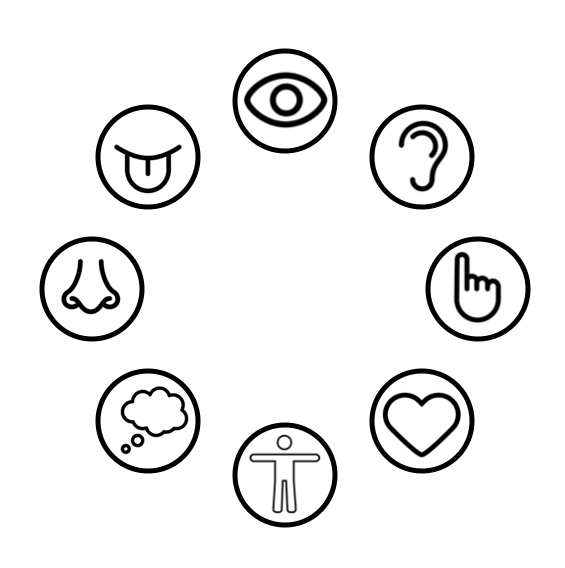
\includegraphics[width=0.8\linewidth]{images/sense-doors.png}
  \caption{The sense doors and bodily sensation. \cite{sense-icons}}
  \label{fig:sense-doors}
\end{figure}

The totality of human experience can be categorized according to the ``sense doors''
listed in Figure~\ref{fig:sense-doors}: The five external sense doors of sight, sound,
taste, smell, and touch are listed at the top. The internal sense door of ``mind'' is
broken down into thought and emotion, second to the bottom. At the very bottom of the
diagram is bodily sensation, the object of meditation in Vipassana.

Once these eight experiences are listed, there is no experience left undescribed. All
human experience from the mundane (imagination, daydreaming, physical pleasures,
physical discomforts, etc.) to the supramundane (out-of-body experiences,
hallucinations, pronounced perceptual time dilation, etc.) are subsets of these seven
sense doors and their reflection in bodily sensation, the eighth.

This concept, that sensory input is ``reflected'' in internal bodily sensation,

Mapping all of sensory experience to these eight categories begs the question of
attention, of awareness: Where does the meditator try to fasten her awareness? Where
is awareness normally? For the average person, awareness jumps around across these
eight categories. Even when one tries to focus on a difficult intellectual problem,
the discomforts of back pain and hunger or the distraction of an irritating sound
would draw attention away from thought, the desired object of attention. Vipassana
meditation asks the meditator to use bodily sensation as a gateway to the other seven
sense experiences. Rather than focusing on sound, focus on the sensation generated in
the body by the ear sense door. Rather than focusing on a thought or emotion, focus
on the sensation in the body generated by that thought or emotion. This is extremely
difficult to do, which is why (for lay people, in most cases) a 10-day silent
residential course \cite{dhamma} is necessary to learn the technique.

\section{The Supramundane Sphere of Experience}

\begin{itemize}
  \item reset frame of reference outside oneself, outside one's own lifetime: ``trees
    for god'' and obvious karma (sidu/booga smoking)
  \item Time: Nat Friedman's blog post?
  \item bible; ``a perfect set of rules''; nature itself <=> perception; ``perfect
    perception (vision)''; inner perception (sensation mirror) --- harris v. peterson
  \item clarification: ``isn't that what makes us human?'' (emotions) --- rather,
    what makes us animal
  \item ``How to Change Your Mind'' --- ego dissolution --- specific advantages?
  \item seeing oneself as aggregate and the path from singular => aggregate
    (neuroscience behind hemispheres)
\end{itemize}


\section*{Acknowledgements}

Thank you to Preethi Govindarajan for reviewing this paper.


\section*{References}

\begin{thebibliography}{99}

\bibitem{sense-icons}
  5 Senses by Daniel Falk from the Noun Project
  \url{https://thenounproject.com/daniel2021/collection/human-body-senses/}
  Thought by Nociconist from the Noun Project
  \url{https://thenounproject.com/search/?q=thought&i=2025873}
  Heart by Rafael Garcia Motta from the Noun Project
  \url{https://thenounproject.com/search/?q=heart&i=807960}
  Body by Makarenko Andrey from the Noun Project
  \url{https://thenounproject.com/search/?q=body&i=789989}
  \textit{The Noun Project}.

\bibitem{mellman2006}
  Mellman, Thomas A.
  \textit{Sleep and Anxiety Disorders.}
  Psychiatric Clinics of North America, Volume 29, Issue 4, Pages 1047-1058, December 2006.
  \url{https://doi.org/10.1016/j.psc.2006.08.005}

\bibitem{staner2003}
  Staner, L.
  \textit{Sleep and anxiety disorders.}
  Dialogues in Clinical Neuroscience, Volume 5(3), Pages 249–258, September 2003.
  PMID: 22033804; PMCID: PMC3181635.

\bibitem{gregory2005}
  Gregory, A.M., Caspi, A., Eley, T.C. et al.
  \textit{Prospective Longitudinal Associations Between Persistent Sleep Problems in
    Childhood and Anxiety and Depression Disorders in Adulthood}
  Journal of Abnormal Child Psychology, Volume 33, Issue 2, pp 157–163, April 2005.
  \url{https://doi.org/10.1007/s10802-005-1824-0}

\bibitem{willis2015}
  Willis, T.A., Gregory, A.M.
  \textit{Anxiety Disorders and Sleep in Children and Adolescents.}
  Sleep Medicine Clinics, Volume 10, Issue 2, Pages 125-131, June 2015.
  \url{https://doi.org/10.1016/j.jsmc.2015.02.002}

\bibitem{hauke2018}
  Hauke G., Kritikos A.
  \textit{Building a Body of Evidence: From Sensation to Emotion and Psychotherapy.}
  Embodiment in Psychotherapy. Springer, Cham.
  ISBN: 978-3-319-92888-3. December 2018.
  \url{https://doi.org/10.1007/978-3-319-92889-0_1}

\bibitem{goenka1999discourses}
  Discourses on satipatthana sutta
%  @article{goenka1999discourses,
%  title={Discourses on satipatthana sutta},
%  author={Goenka, Satya Narayan},
%  journal={Igatpuri, Maharashtra, India: Vipassana Research Institute},
%  year={1999}
%}

\bibitem{nagendra2012}
  Nagendra R.P., Maruthai N., Kutty B.M.
  \textit{Meditation and its regulatory role on sleep.}
  Frontiers in Neurology, 3:54, April 2012.
  \url{https://doi.org/10.3389/fneur.2012.00054}

\bibitem{maruthai2016senior}
  Maruthai N., Nagendra R.P., Sasidharan A., Srikumar S., Datta K., Uchida S., Kutty B.M.
  \textit{Senior Vipassana Meditation practitioners exhibit distinct REM sleep
    organization from that of novice meditators and healthy controls.}
  International Review of Psychiatry, Volume 28(3), Pages 279-287, April 2016.
  \url{https://doi.org/10.3109/09540261.2016.1159949}

\bibitem{black2015}
  Black D.S., O’Reilly G.A., Olmstead R., Breen E.C., Irwin M.R.
  \textit{Mindfulness Meditation and Improvement in Sleep Quality and Daytime Impairment
    Among Older Adults With Sleep Disturbances: A Randomized Clinical Trial.}
  JAMA Internal Medicine, Volume 175(4), Pages 494–501, 2015.

\bibitem{uclamaps}
  Mindful Awareness Practices (MAPs) Classes
  \url{https://www.uclahealth.org/marc/maps-classes}

\bibitem{dhamma}
  Vipassana International Academy
  \url{https://www.dhamma.org}
  \textit{Vipassana Meditation Website}


\end{thebibliography}

\end{document}
